\documentclass[UTF8,fontset=none,11pt]{ctexart}
\usepackage[a4paper,margin=2.05cm]{geometry}
\usepackage{amsmath,amssymb}
\usepackage{enumitem}
\usepackage[table]{xcolor}
\usepackage{booktabs}
\usepackage{array}
\usepackage{longtable}
\usepackage{tikz}
\usepackage{graphicx}
\usepackage{hyperref}
\usetikzlibrary{positioning,arrows.meta,shapes.geometric,fit,backgrounds,calc}

\setCJKmainfont[AutoFakeSlant=0.18]{PingFang SC}
\setCJKsansfont[AutoFakeSlant=0.18]{PingFang SC}
\setCJKmonofont[AutoFakeSlant=0.18]{PingFang SC}

\hypersetup{
  colorlinks=true,
  linkcolor=blue!55!black,
  urlcolor=blue!55!black,
  citecolor=blue!55!black,
  pdftitle={编译原理语法分析知识点文档},
  pdfauthor={Trae AI}
}

\setlength{\parindent}{0pt}
\setlength{\parskip}{0.55em}
\setlist[itemize]{leftmargin=1.8em,itemsep=0.22em,topsep=0.25em}
\setlist[enumerate]{leftmargin=2.0em,itemsep=0.28em,topsep=0.3em}
\renewcommand{\arraystretch}{1.18}
\setlength{\emergencystretch}{3em}
\sloppy

\definecolor{defrule}{RGB}{25,92,140}
\definecolor{noterule}{RGB}{120,80,15}
\definecolor{warnrule}{RGB}{160,50,45}
\definecolor{softblue}{RGB}{235,246,255}
\definecolor{softgreen}{RGB}{236,250,240}
\definecolor{softyellow}{RGB}{255,249,230}
\definecolor{softred}{RGB}{255,241,239}
\definecolor{graytext}{RGB}{95,95,95}
\newcolumntype{L}[1]{>{\raggedright\arraybackslash}p{#1}}

\newenvironment{defbox}[1][]{%
  \par\medskip\noindent{\color{defrule}\rule{\linewidth}{1.1pt}}\par\nopagebreak
  \noindent{\bfseries\color{defrule}#1}\par\nopagebreak\smallskip}%
  {\par\nopagebreak\smallskip\noindent{\color{defrule}\rule{\linewidth}{0.4pt}}\par\medskip}
\newenvironment{notebox}[1][]{%
  \par\medskip\noindent{\color{noterule}\rule{\linewidth}{1.1pt}}\par\nopagebreak
  \noindent{\bfseries\color{noterule}#1}\par\nopagebreak\smallskip}%
  {\par\nopagebreak\smallskip\noindent{\color{noterule}\rule{\linewidth}{0.4pt}}\par\medskip}
\newenvironment{warnbox}[1][]{%
  \par\medskip\noindent{\color{warnrule}\rule{\linewidth}{1.1pt}}\par\nopagebreak
  \noindent{\bfseries\color{warnrule}#1}\par\nopagebreak\smallskip}%
  {\par\nopagebreak\smallskip\noindent{\color{warnrule}\rule{\linewidth}{0.4pt}}\par\medskip}

\newcommand{\eps}{\varepsilon}
\newcommand{\FIRST}{\operatorname{FIRST}}
\newcommand{\FOLLOW}{\operatorname{FOLLOW}}
\newcommand{\CLOSURE}{\operatorname{CLOSURE}}
\newcommand{\GOTO}{\operatorname{GOTO}}
\newcommand{\ACTION}{\operatorname{ACTION}}
\newcommand{\LL}{\mathrm{LL}}
\newcommand{\LR}{\mathrm{LR}}
\newcommand{\SLR}{\mathrm{SLR}}
\newcommand{\LALR}{\mathrm{LALR}}

\tikzset{
  flow/.style={rectangle,rounded corners,draw=defrule,thick,align=center,minimum width=2.7cm,minimum height=0.85cm,fill=softblue},
  smallflow/.style={rectangle,rounded corners,draw=defrule,align=center,minimum width=2.25cm,minimum height=0.72cm,fill=softblue},
  warnflow/.style={rectangle,rounded corners,draw=warnrule,align=center,minimum width=2.4cm,minimum height=0.72cm,fill=softred},
  goodflow/.style={rectangle,rounded corners,draw=green!45!black,align=center,minimum width=2.4cm,minimum height=0.72cm,fill=softgreen},
  state/.style={circle,draw=black,thick,minimum size=8mm,inner sep=0pt},
  itemstate/.style={rectangle,rounded corners,draw=black,thick,align=left,inner sep=4pt,fill=white},
  edge/.style={-{Stealth[length=2.2mm]},thick}
}

\title{\bfseries 编译原理语法分析知识点文档\\从 CFG、LL 到 LR 族与错误恢复}
\author{面向复习与系统掌握的中文技术笔记}
\date{\today}

\begin{document}
\maketitle
\tableofcontents
\newpage

\section*{阅读导引}
\addcontentsline{toc}{section}{阅读导引}

语法分析是编译器前端的核心阶段。词法分析器把字符流切成 token，语法分析器根据语言文法判断 token 序列是否构成合法程序结构，并输出 parse tree 或 AST，供语义分析和中间代码生成使用。

\begin{center}
\resizebox{\linewidth}{!}{
\begin{tikzpicture}[node distance=1.0cm]
  \node[flow] (src) {源代码\\字符流};
  \node[flow,right=of src] (lex) {词法分析\\Token Stream};
  \node[flow,right=of lex] (parse) {语法分析\\Parse Tree / AST};
  \node[flow,right=of parse] (sem) {语义分析\\类型/符号表};
  \node[flow,right=of sem] (ir) {中间代码\\IR};
  \draw[edge] (src) -- (lex);
  \draw[edge] (lex) -- (parse);
  \draw[edge] (parse) -- (sem);
  \draw[edge] (sem) -- (ir);
\end{tikzpicture}
}
\end{center}

\begin{notebox}[总览]
语法分析的主线是：用上下文无关文法描述语言结构；用自上而下或自下而上的算法识别句子；用 LL/LR 表驱动方法把分析过程机械化；用错误恢复机制在遇到语法错误时尽量继续分析。
\end{notebox}

\section{语法分析基本概念}

\subsection{语法分析器的职责}

\begin{defbox}[语法分析]
语法分析（syntax analysis / parsing）读取 token 序列，依据上下文无关文法判断其结构是否合法，并构造语法结构表示，通常是 parse tree 或 AST。
\end{defbox}

语法分析器主要完成：

\begin{itemize}
  \item 验证 token 序列是否符合语言文法。
  \item 在合法时构造程序结构，如表达式、语句、声明、函数体。
  \item 在非法时报告语法错误，并尽可能恢复继续分析。
  \item 为后续语义分析提供结构化输入。
\end{itemize}

词法分析只能识别局部模式，例如标识符、数字、关键字；语法分析处理嵌套和递归结构，例如括号匹配、表达式优先级、语句块、函数定义。

\subsection{分析方法分类}

\begin{center}
\resizebox{\linewidth}{!}{
\begin{tikzpicture}[node distance=0.9cm]
  \node[flow] (parser) {Parser\\语法分析器};
  \node[flow,below left=1.0cm and 1.1cm of parser] (td) {Top-down\\自上而下};
  \node[flow,below right=1.0cm and 1.1cm of parser] (bu) {Bottom-up\\自下而上};
  \node[smallflow,below left=0.9cm and -0.15cm of td] (rd) {递归下降\\RDP};
  \node[smallflow,below right=0.9cm and -0.15cm of td] (ll) {LL 分析\\预测分析};
  \node[smallflow,below left=0.9cm and -0.15cm of bu] (sr) {移进-规约\\Shift-Reduce};
  \node[smallflow,below right=0.9cm and -0.15cm of bu] (lr) {LR 族\\SLR/LR(1)/LALR};
  \draw[edge] (parser) -- (td);
  \draw[edge] (parser) -- (bu);
  \draw[edge] (td) -- (rd);
  \draw[edge] (td) -- (ll);
  \draw[edge] (bu) -- (sr);
  \draw[edge] (bu) -- (lr);
\end{tikzpicture}
}
\end{center}

\begin{longtable}{L{0.18\linewidth}L{0.35\linewidth}L{0.37\linewidth}}
\toprule
类别 & 思路 & 典型算法 \\
\midrule
自上而下 & 从开始符号出发，尝试推导出输入串 & 递归下降、LL(1)、LL(k) \\
自下而上 & 从输入串出发，逐步规约回开始符号 & shift-reduce、LR(0)、SLR、LR(1)、LALR \\
\bottomrule
\end{longtable}

\section{上下文无关文法 CFG}

\subsection{CFG 四元组}

\begin{defbox}[上下文无关文法]
上下文无关文法 CFG 是四元组
\[
G=(V,T,P,S).
\]
\(V\) 是非终结符集合，\(T\) 是终结符集合，\(P\) 是产生式集合，\(S\) 是开始符号。
\end{defbox}

\begin{center}
\begin{tikzpicture}[node distance=1.0cm]
  \node[flow] (g) {CFG\\\(G=(V,T,P,S)\)};
  \node[smallflow,below left=0.75cm and 1.2cm of g] (v) {\(V\)\\非终结符};
  \node[smallflow,below left=0.75cm and -0.2cm of g] (t) {\(T\)\\终结符};
  \node[smallflow,below right=0.75cm and -0.2cm of g] (p) {\(P\)\\产生式};
  \node[smallflow,below right=0.75cm and 1.2cm of g] (s) {\(S\)\\开始符号};
  \draw[edge] (g) -- (v);
  \draw[edge] (g) -- (t);
  \draw[edge] (g) -- (p);
  \draw[edge] (g) -- (s);
\end{tikzpicture}
\end{center}

表达式文法示例：
\[
\begin{aligned}
E &\to E+T\mid T\\
T &\to T*F\mid F\\
F &\to (E)\mid id
\end{aligned}
\]
其中 \(E,T,F\) 是非终结符，\(id,+,*,(,)\) 是终结符。

\subsection{推导、句型、句子与语言}

\begin{itemize}
  \item 推导：反复用产生式右部替换左部非终结符的过程。
  \item 句型：从开始符号可推导出的任意符号串，可包含非终结符。
  \item 句子：只含终结符的句型。
  \item 文法语言：所有可由开始符号推导出的句子集合。
\end{itemize}

最左推导每次替换最左非终结符；最右推导每次替换最右非终结符。自上而下分析常对应最左推导；自下而上分析常对应最右推导的逆过程。

\subsection{分析树与 AST}

\begin{defbox}[Parse Tree]
分析树把推导过程表示成树：根是开始符号，内部节点是非终结符，叶子从左到右组成输入串。
\end{defbox}

\begin{center}
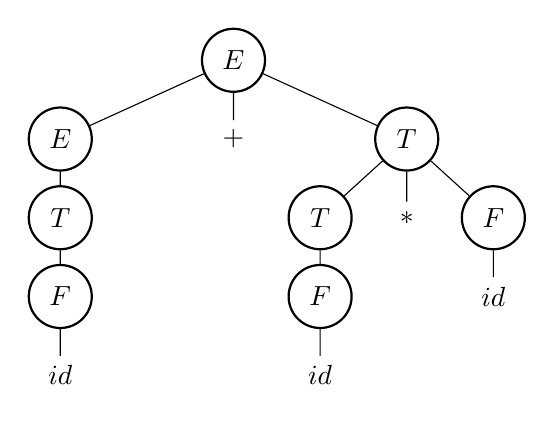
\begin{tikzpicture}[level distance=1.0cm,
  level 1/.style={sibling distance=2.2cm},
  level 2/.style={sibling distance=1.1cm},
  every node/.style={align=center}]
  \node[state] {\(E\)}
    child {node[state] {\(E\)}
      child {node[state] {\(T\)}
        child {node[state] {\(F\)}
          child {node {\(id\)}}}}}
    child {node {\(+\)}}
    child {node[state] {\(T\)}
      child {node[state] {\(T\)}
        child {node[state] {\(F\)}
          child {node {\(id\)}}}}
      child {node {\(*\)}}
      child {node[state] {\(F\)}
        child {node {\(id\)}}}};
\end{tikzpicture}
\end{center}

\begin{defbox}[AST]
抽象语法树 AST 去掉多余语法细节，只保留程序语义结构。例如括号节点、单一产生式链条通常会被省略。
\end{defbox}

Parse tree 更适合证明输入符合文法；AST 更适合后续语义分析和代码生成。

\subsection{二义性与消歧}

\begin{defbox}[二义性]
若某个句子在同一文法下有两棵不同分析树，或有两个不同最左/最右推导，则该文法是二义的。
\end{defbox}

典型二义文法：
\[
E\to E+E\mid E*E\mid (E)\mid id.
\]
句子 \(id+id*id\) 既可理解为 \((id+id)*id\)，也可理解为 \(id+(id*id)\)。

常用消歧方法：

\begin{itemize}
  \item 重写文法，把优先级编码到非终结符层次中。
  \item 使用结合性规则，如加法左结合。
  \item 在 parser generator 中声明优先级和结合性。
\end{itemize}

表达式的非二义文法常写成：
\[
E\to E+T\mid T,\quad T\to T*F\mid F,\quad F\to (E)\mid id.
\]
这里 \(T\) 比 \(E\) 更靠近叶子，表示乘法优先级高于加法。

\section{文法变换与 FIRST/FOLLOW}

\subsection{左递归}

\begin{defbox}[左递归]
若非终结符 \(A\) 可推导出以自身开头的句型，即 \(A\Rightarrow^+ A\alpha\)，则 \(A\) 存在左递归。直接左递归形如 \(A\to A\alpha\mid\beta\)。
\end{defbox}

左递归会导致递归下降分析无限递归。直接左递归消除：
\[
A\to A\alpha_1\mid\cdots\mid A\alpha_m\mid\beta_1\mid\cdots\mid\beta_n
\]
改写为：
\[
A\to \beta_1A'\mid\cdots\mid\beta_nA'
\]
\[
A'\to \alpha_1A'\mid\cdots\mid\alpha_mA'\mid\eps.
\]

\begin{center}
\begin{tikzpicture}[node distance=1.1cm]
  \node[warnflow] (before) {\(A\to A\alpha\mid\beta\)\\左递归};
  \node[flow,right=of before] (rewrite) {引入 \(A'\)\\把重复放到右侧};
  \node[goodflow,right=of rewrite] (after) {\(A\to\beta A'\)\\\(A'\to\alpha A'\mid\eps\)};
  \draw[edge] (before) -- (rewrite);
  \draw[edge] (rewrite) -- (after);
\end{tikzpicture}
\end{center}

\subsection{左因子提取}

若多个候选式有公共前缀：
\[
A\to \alpha\beta_1\mid\alpha\beta_2,
\]
预测分析器看到 \(\alpha\) 时无法立刻选择。提取左因子：
\[
A\to \alpha A',\quad A'\to \beta_1\mid\beta_2.
\]

通俗地说：先吃掉共同开头，再根据后续 token 作选择。

\subsection{FIRST 集}

\begin{defbox}[FIRST]
\(\FIRST(\alpha)\) 是可能出现在 \(\alpha\) 推导结果最前面的终结符集合。若 \(\alpha\Rightarrow^*\eps\)，则 \(\eps\in\FIRST(\alpha)\)。
\end{defbox}

计算规则：

\begin{itemize}
  \item 若 \(X\) 是终结符，则 \(\FIRST(X)=\{X\}\)。
  \item 若 \(A\to\eps\)，则 \(\eps\in\FIRST(A)\)。
  \item 若 \(A\to X_1X_2\cdots X_n\)，先把 \(\FIRST(X_1)-\{\eps\}\) 加入 \(\FIRST(A)\)；若 \(X_1\) 可为空，再看 \(X_2\)，依此类推。
  \item 若所有 \(X_i\) 都可为空，则 \(\eps\in\FIRST(A)\)。
\end{itemize}

\subsection{FOLLOW 集}

\begin{defbox}[FOLLOW]
\(\FOLLOW(A)\) 是在某个句型中可能紧跟在非终结符 \(A\) 后面的终结符集合。若 \(A\) 可出现在输入末尾，则 \(\$\in\FOLLOW(A)\)。
\end{defbox}

计算规则：

\begin{itemize}
  \item 对开始符号 \(S\)，\(\$\in\FOLLOW(S)\)。
  \item 若 \(A\to\alpha B\beta\)，则把 \(\FIRST(\beta)-\{\eps\}\) 加入 \(\FOLLOW(B)\)。
  \item 若 \(A\to\alpha B\beta\) 且 \(\beta\Rightarrow^*\eps\)，则把 \(\FOLLOW(A)\) 加入 \(\FOLLOW(B)\)。
  \item 若 \(A\to\alpha B\)，则把 \(\FOLLOW(A)\) 加入 \(\FOLLOW(B)\)。
\end{itemize}

\begin{center}
\begin{tikzpicture}[node distance=1.0cm]
  \node[flow] (first) {计算 FIRST\\看右部开头};
  \node[flow,right=of first] (follow) {计算 FOLLOW\\看符号后面};
  \node[flow,right=of follow] (table) {构造 LL 表\\或 SLR 规约列};
  \draw[edge] (first) -- (follow);
  \draw[edge] (follow) -- (table);
\end{tikzpicture}
\end{center}

\section{自上而下分析与 LL}

\subsection{自上而下分析思想}

自上而下分析从开始符号出发，试图逐步展开非终结符，使叶子序列匹配输入。它模拟最左推导。

\begin{center}
\begin{tikzpicture}[node distance=1.0cm]
  \node[flow] (start) {开始符号 \(S\)};
  \node[flow,right=of start] (choose) {选择产生式\\展开最左非终结符};
  \node[flow,right=of choose] (match) {匹配当前 token};
  \node[flow,right=of match] (done) {全部匹配\\接受};
  \node[warnflow,below=0.9cm of choose] (err) {无可用产生式\\或终结符不匹配};
  \draw[edge] (start) -- (choose);
  \draw[edge] (choose) -- (match);
  \draw[edge] (match) -- (done);
  \draw[edge] (choose) -- (err);
\end{tikzpicture}
\end{center}

\subsection{递归下降分析}

递归下降分析为每个非终结符写一个函数。函数根据 lookahead token 选择产生式，并递归调用其他非终结符函数。

优点：

\begin{itemize}
  \item 直观，容易手写。
  \item 错误信息可定制。
  \item 适合工程语言的部分语法。
\end{itemize}

缺点：

\begin{itemize}
  \item 左递归会无限递归。
  \item 若文法不是预测性的，可能需要回溯。
  \item 回溯会降低效率，也会让错误定位变差。
\end{itemize}

\subsection{LL(1) 文法条件}

\begin{defbox}[LL(1)]
LL(1) 表示从左到右扫描输入（Left-to-right），构造最左推导（Leftmost derivation），只看 1 个向前看符号。
\end{defbox}

对同一非终结符的任意两个候选式 \(A\to\alpha\mid\beta\)，LL(1) 要求：

\[
\FIRST(\alpha)\cap\FIRST(\beta)=\emptyset.
\]

若 \(\eps\in\FIRST(\alpha)\)，还要：
\[
\FIRST(\beta)\cap\FOLLOW(A)=\emptyset.
\]

直观解释：看一个 token 时，分析器必须唯一知道选哪条产生式。

\subsection{预测分析表构造}

对每条产生式 \(A\to\alpha\)：

\begin{enumerate}
  \item 对每个 \(a\in\FIRST(\alpha)-\{\eps\}\)，把 \(A\to\alpha\) 填入 \(M[A,a]\)。
  \item 若 \(\eps\in\FIRST(\alpha)\)，对每个 \(b\in\FOLLOW(A)\)，把 \(A\to\alpha\) 填入 \(M[A,b]\)。
  \item 未填的格子表示语法错误。
\end{enumerate}

\begin{center}
\begin{tikzpicture}[node distance=0.9cm]
  \node[flow] (prod) {产生式\\\(A\to\alpha\)};
  \node[flow,right=of prod] (first) {填 FIRST(\(\alpha\))\\对应列};
  \node[flow,right=of first] (eps) {若可推出 \(\eps\)\\填 FOLLOW(A)};
  \node[flow,right=of eps] (m) {得到预测\\分析表 M};
  \draw[edge] (prod) -- (first);
  \draw[edge] (first) -- (eps);
  \draw[edge] (eps) -- (m);
\end{tikzpicture}
\end{center}

\subsection{非递归 LL(1) 分析器}

表驱动 LL(1) parser 使用分析栈、输入缓冲区和预测分析表。

\begin{center}
\resizebox{\linewidth}{!}{
\begin{tikzpicture}[node distance=1.0cm]
  \node[flow] (input) {输入缓冲区\\token... \(\$\)};
  \node[flow,right=of input] (driver) {预测分析器\\表驱动程序};
  \node[flow,above=0.8cm of driver] (stack) {分析栈\\\(\$S\)};
  \node[flow,right=of driver] (table) {LL(1) 表\\\(M[A,a]\)};
  \node[goodflow,right=of table] (out) {产生式序列\\或 AST 动作};
  \draw[edge] (input) -- (driver);
  \draw[edge] (stack) -- (driver);
  \draw[edge] (table) -- (driver);
  \draw[edge] (driver) -- (out);
\end{tikzpicture}
}
\end{center}

运行规则：

\begin{itemize}
  \item 若栈顶是终结符且等于当前输入 token，则弹栈并读下一个 token。
  \item 若栈顶是非终结符 \(A\)，查表 \(M[A,a]\)。
  \item 若查到 \(A\to X_1\cdots X_n\)，弹出 \(A\)，把 \(X_n,\ldots,X_1\) 反向压栈。
  \item 若查表为空或终结符不匹配，报告错误。
\end{itemize}

\section{自下而上分析与移进-规约}

\subsection{自下而上分析思想}

自下而上分析从输入串出发，把右部逐步规约成左部，最终规约为开始符号。它对应最右推导的逆过程。

\begin{center}
\begin{tikzpicture}[node distance=1.0cm]
  \node[flow] (input) {输入 token};
  \node[flow,right=of input] (shift) {移进\\shift};
  \node[flow,right=of shift] (reduce) {发现句柄\\reduce};
  \node[flow,right=of reduce] (start) {规约到 \(S\)\\接受};
  \draw[edge] (input) -- (shift);
  \draw[edge] (shift) -- (reduce);
  \draw[edge] (reduce) to[bend left=25] node[above]{继续} (shift);
  \draw[edge] (reduce) -- (start);
\end{tikzpicture}
\end{center}

\subsection{短语、直接短语、句柄}

\begin{defbox}[句柄]
句柄是在某个右句型中，下一步应被规约的产生式右部。把句柄规约为左部，正好逆转最右推导的一步。
\end{defbox}

移进-规约 parser 的任务可以理解为：不断把输入读入栈，在栈顶找到句柄后规约。

\subsection{移进-规约动作}

\begin{longtable}{L{0.16\linewidth}L{0.72\linewidth}}
\toprule
动作 & 含义 \\
\midrule
Shift & 把当前输入符号移入栈，读下一个 token \\
Reduce & 若栈顶匹配某产生式右部 \(\beta\)，用左部 \(A\) 替换 \(\beta\) \\
Accept & 输入已读完，栈中为开始符号，分析成功 \\
Error & 没有合法动作，报告语法错误 \\
\bottomrule
\end{longtable}

\subsection{冲突}

\begin{warnbox}[Shift-reduce conflict]
同一状态、同一 lookahead 下既可以移进，也可以规约，称为移进-规约冲突。表达式优先级和 dangling else 常导致此问题。
\end{warnbox}

\begin{warnbox}[Reduce-reduce conflict]
同一状态、同一 lookahead 下可以按两条不同产生式规约，称为规约-规约冲突。它通常说明文法或语义设计存在更严重的二义性。
\end{warnbox}

\section{LR 分析通用框架}

\subsection{LR(k) 含义}

\begin{defbox}[LR(k)]
LR(k) 表示从左到右扫描输入（Left-to-right），构造最右推导的逆过程（Rightmost derivation in reverse），使用 \(k\) 个 lookahead 符号。
\end{defbox}

LR 分析能力强于 LL，能处理很多左递归文法，也更适合自动生成 parser。

\subsection{LR 分析器结构}

LR parser 维护状态栈和符号栈，依据 ACTION/GOTO 表决定动作。

\begin{center}
\resizebox{\linewidth}{!}{
\begin{tikzpicture}[node distance=1.0cm]
  \node[flow] (input) {输入\\\(a_1a_2\cdots\$\)};
  \node[flow,right=of input] (driver) {LR 驱动程序};
  \node[flow,above=0.8cm of driver] (stack) {状态栈/符号栈\\\(s_0X_1s_1\cdots\)};
  \node[flow,right=of driver] (act) {ACTION 表\\shift/reduce/accept};
  \node[flow,below=0.8cm of act] (goto) {GOTO 表\\非终结符转移};
  \node[goodflow,right=of act] (tree) {规约序列\\Parse Tree / AST};
  \draw[edge] (input) -- (driver);
  \draw[edge] (stack) -- (driver);
  \draw[edge] (act) -- (driver);
  \draw[edge] (goto) -- (driver);
  \draw[edge] (driver) -- (tree);
\end{tikzpicture}
}
\end{center}

动作规则：

\begin{itemize}
  \item \(\ACTION[s,a]=shift\ t\)：移进当前输入 \(a\)，压入状态 \(t\)。
  \item \(\ACTION[s,a]=reduce\ A\to\beta\)：弹出 \(|\beta|\) 个符号和状态，再按 \(\GOTO[s',A]\) 压入新状态。
  \item \(\ACTION[s,\$]=accept\)：接受。
  \item 空表项：错误。
\end{itemize}

\section{LR(0)、SLR、LR(1)、LALR}

\subsection{LR(0) 项与项目集族}

\begin{defbox}[LR(0) item]
LR(0) 项是在产生式右部某位置加点，例如 \(A\to\alpha\cdot\beta\)。点表示右部已经识别到的位置。
\end{defbox}

例子：

\[
E\to E+\cdot T
\]
表示已经看到 \(E+\)，接下来希望看到 \(T\)。

\subsection{CLOSURE 与 GOTO}

\begin{defbox}[CLOSURE]
若项目集中有 \(A\to\alpha\cdot B\beta\)，说明接下来可能识别非终结符 \(B\)。因此要把 \(B\) 的所有产生式 \(B\to\gamma\) 对应项目 \(B\to\cdot\gamma\) 加入集合，直到不再变化。
\end{defbox}

\begin{defbox}[GOTO]
\(\GOTO(I,X)\) 表示项目集 \(I\) 在识别符号 \(X\) 后到达的新项目集。做法是把所有点前为 \(X\) 的项目点右移一位，再取 CLOSURE。
\end{defbox}

\begin{center}
\resizebox{\linewidth}{!}{
\begin{tikzpicture}[node distance=0.9cm]
  \node[flow] (aug) {增广文法\\\(S'\to S\)};
  \node[flow,right=of aug] (i0) {\(I_0=\CLOSURE(S'\to\cdot S)\)};
  \node[flow,right=of i0] (goto) {对每个符号\\计算 GOTO};
  \node[flow,right=of goto] (dfa) {得到 LR(0)\\项目 DFA};
  \node[flow,right=of dfa] (table) {构造\\ACTION/GOTO};
  \draw[edge] (aug) -- (i0);
  \draw[edge] (i0) -- (goto);
  \draw[edge] (goto) -- (dfa);
  \draw[edge] (dfa) -- (table);
\end{tikzpicture}
}
\end{center}

\subsection{LR(0) 表构造}

对每个项目集状态 \(I_i\)：

\begin{itemize}
  \item 若 \(A\to\alpha\cdot a\beta\) 且 \(a\) 是终结符，\(\GOTO(I_i,a)=I_j\)，则 \(\ACTION[i,a]=shift\ j\)。
  \item 若 \(A\to\alpha\cdot\) 是完成项，且 \(A\ne S'\)，则对所有终结符填入 \(reduce\ A\to\alpha\)。
  \item 若 \(S'\to S\cdot\)，则 \(\ACTION[i,\$]=accept\)。
  \item 若 \(\GOTO(I_i,A)=I_j\) 且 \(A\) 是非终结符，则 \(\GOTO[i,A]=j\)。
\end{itemize}

LR(0) 没有 lookahead，完成项会在所有终结符上规约，因此容易冲突。

\subsection{SLR(1)}

\begin{defbox}[SLR(1)]
SLR 使用 LR(0) 项目集构造状态，但规约动作只填在 \(\FOLLOW(A)\) 对应列中。它比 LR(0) 更保守，也能减少冲突。
\end{defbox}

SLR 规约规则：

若状态 \(i\) 中有完成项 \(A\to\alpha\cdot\)，则只对
\[
a\in\FOLLOW(A)
\]
填入
\[
\ACTION[i,a]=reduce\ A\to\alpha.
\]

SLR 的优点是简单；缺点是 FOLLOW 集是全局近似，可能把不该规约的 lookahead 也包含进来，因此分析能力有限。

\subsection{LR(1)}

\begin{defbox}[LR(1) item]
LR(1) 项形如
\[
[A\to\alpha\cdot\beta,\ a],
\]
其中 \(a\) 是 lookahead。它表示当未来看到 \(a\) 时，完成的 \(A\) 才允许规约。
\end{defbox}

LR(1) 的 Closure 会传播 lookahead：

若有
\[
[A\to\alpha\cdot B\beta,\ a],
\]
则对 \(B\to\gamma\)，加入
\[
[B\to\cdot\gamma,\ b]\quad b\in\FIRST(\beta a).
\]

LR(1) 优点是信息精确，分析能力强；缺点是状态数可能很多。

\subsection{LALR(1)}

\begin{defbox}[LALR(1)]
LALR 把 LR(1) 中 LR(0) 核心相同的状态合并，并合并 lookahead 集合。它通常保持接近 LR(1) 的分析能力，同时状态数接近 SLR。
\end{defbox}

关系图：

\begin{center}
\begin{tikzpicture}[node distance=0.9cm]
  \node[flow] (lr0) {LR(0)\\最弱/最小};
  \node[flow,right=of lr0] (slr) {SLR(1)\\FOLLOW 限制};
  \node[flow,right=of slr] (lalr) {LALR(1)\\合并 LR(1) 核心};
  \node[flow,right=of lalr] (lr1) {LR(1)\\最强/状态多};
  \draw[edge] (lr0) -- node[above]{能力增强} (slr);
  \draw[edge] (slr) -- (lalr);
  \draw[edge] (lalr) -- (lr1);
\end{tikzpicture}
\end{center}

更准确地说，文法类包含关系通常为：
\[
LR(0)\subset SLR(1)\subset LALR(1)\subset LR(1).
\]
状态规模大致为：
\[
LR(0)\approx SLR(1)\approx LALR(1) < LR(1).
\]

\begin{warnbox}[LALR 的风险]
合并 LR(1) 状态可能引入 reduce-reduce conflict，但不会引入新的 shift-reduce conflict。LALR 也可能比 LR(1) 更晚发现错误。
\end{warnbox}

\section{LL 与 LR 对比}

\begin{longtable}{L{0.18\linewidth}L{0.36\linewidth}L{0.36\linewidth}}
\toprule
维度 & LL & LR \\
\midrule
方向 & 自上而下，从开始符号推导输入 & 自下而上，从输入规约到开始符号 \\
推导关系 & 构造最左推导 & 构造最右推导的逆过程 \\
典型实现 & 递归下降、预测分析表 & shift-reduce、ACTION/GOTO 表 \\
文法要求 & 不支持左递归，常需左因子提取 & 可处理很多左递归文法 \\
错误定位 & 通常较早、较直观 & 通常能准确知道无法继续的状态 \\
分析能力 & 较弱，LL(1) 要求严格 & 较强，LR(1) 能处理更大文法类 \\
工程使用 & 手写 parser 常用 & parser generator 常用 \\
\bottomrule
\end{longtable}

直观理解：

\begin{itemize}
  \item LL 是“先猜结构，再验证输入”。
  \item LR 是“先读输入，等证据足够后再确认结构”。
  \item LR 更晚做决定，因此能处理更多文法。
\end{itemize}

\section{语法错误恢复}

\subsection{错误恢复目标}

语法分析遇到错误时不能只崩溃退出。好的 parser 应该：

\begin{itemize}
  \item 报告清晰的位置和原因。
  \item 避免一处错误引发大量伪错误。
  \item 尽量跳过错误片段继续分析后续代码。
  \item 保证恢复过程不会陷入死循环。
\end{itemize}

\subsection{常见错误恢复策略}

\begin{longtable}{L{0.22\linewidth}L{0.36\linewidth}L{0.32\linewidth}}
\toprule
策略 & 做法 & 特点 \\
\midrule
Panic-mode & 跳过输入直到同步符号，如分号、右括号、关键字 & 简单稳健，但可能跳过较多内容 \\
Phrase-level & 在局部插入、删除或替换少量 token & 错误信息更友好，但规则需谨慎设计 \\
Error productions & 文法中显式加入常见错误产生式 & 能针对常见错误给精确提示 \\
Global correction & 寻找最小编辑距离修复方案 & 理论漂亮，实际代价高，较少用于工程 \\
\bottomrule
\end{longtable}

\subsection{Panic-mode 流程}

\begin{center}
\begin{tikzpicture}[node distance=0.9cm]
  \node[flow] (err) {检测到错误};
  \node[flow,right=of err] (report) {报告错误\\记录位置};
  \node[warnflow,right=of report] (skip) {跳过 token\\直到同步符号};
  \node[flow,right=of skip] (sync) {调整栈/状态\\恢复上下文};
  \node[goodflow,right=of sync] (go) {继续分析};
  \draw[edge] (err) -- (report);
  \draw[edge] (report) -- (skip);
  \draw[edge] (skip) -- (sync);
  \draw[edge] (sync) -- (go);
\end{tikzpicture}
\end{center}

常见同步符号：

\begin{itemize}
  \item 语句结束符：\texttt{;}。
  \item 块边界：\texttt{\{}、\texttt{\}}。
  \item 结构关键字：\texttt{if}、\texttt{while}、\texttt{return}。
  \item FOLLOW 集中的符号。
\end{itemize}

\subsection{LL 与 LR 中的错误恢复}

LL 表驱动分析中，可在空表项 \(M[A,a]\) 放入 synch 标记。当栈顶为非终结符 \(A\)，当前输入为 \(a\)，且 \(a\in\FOLLOW(A)\) 时，可弹出 \(A\)，认为缺失了某个结构。

LR 分析中，若 ACTION 表为空，可：

\begin{itemize}
  \item 弹出状态直到某个状态可转移到错误恢复非终结符。
  \item 跳过输入直到同步 token。
  \item 移入特殊 error 符号，再继续分析。
\end{itemize}

\section{综合示例：表达式文法从 LL 到 LR}

原始表达式文法：
\[
E\to E+T\mid T,\quad T\to T*F\mid F,\quad F\to (E)\mid id.
\]

它适合 LR，因为左递归表达左结合自然；但不适合递归下降。改写为 LL(1)：
\[
\begin{aligned}
E&\to TE'\\
E'&\to +TE'\mid\eps\\
T&\to FT'\\
T'&\to *FT'\mid\eps\\
F&\to (E)\mid id
\end{aligned}
\]

\begin{center}
\resizebox{\linewidth}{!}{
\begin{tikzpicture}[node distance=1.0cm]
  \node[warnflow] (orig) {左递归表达式文法\\适合 LR};
  \node[flow,right=of orig] (elim) {消除左递归\\引入 \(E',T'\)};
  \node[flow,right=of elim] (first) {计算 FIRST/FOLLOW};
  \node[goodflow,right=of first] (ll) {构造 LL(1) 表\\递归下降可用};
  \draw[edge] (orig) -- (elim);
  \draw[edge] (elim) -- (first);
  \draw[edge] (first) -- (ll);
\end{tikzpicture}
}
\end{center}

核心 FIRST/FOLLOW：

\begin{center}
\begin{tabular}{c|c|c}
\toprule
非终结符 & FIRST & FOLLOW \\
\midrule
\(E\) & \(\{(,id\}\) & \(\{\$,)\}\) \\
\(E'\) & \(\{+,\eps\}\) & \(\{\$,)\}\) \\
\(T\) & \(\{(,id\}\) & \(\{+, \$, )\}\) \\
\(T'\) & \(\{*,\eps\}\) & \(\{+, \$, )\}\) \\
\(F\) & \(\{(,id\}\) & \(\{*, +, \$, )\}\) \\
\bottomrule
\end{tabular}
\end{center}

这说明同一种语言可用不同文法服务不同 parser：LR 文法更自然表达左结合；LL 文法更适合预测分析。

\section{复习清单}

\begin{itemize}
  \item 能写出 CFG 四元组，并区分终结符、非终结符、句型、句子、语言。
  \item 能解释最左推导、最右推导、parse tree、AST 和二义性。
  \item 能消除直接左递归、提取左因子。
  \item 能计算 FIRST 和 FOLLOW，并据此构造 LL(1) 表。
  \item 能解释递归下降、预测分析和 LL(1) 条件。
  \item 能解释 shift、reduce、handle、viable prefix 和冲突。
  \item 能构造 LR(0) 项目、CLOSURE、GOTO 和 ACTION/GOTO 表。
  \item 能说明 LR(0)、SLR、LR(1)、LALR 的区别和包含关系。
  \item 能比较 LL 与 LR 的优缺点。
  \item 能说明 panic-mode、phrase-level、error productions 和 global correction。
\end{itemize}

\section*{结语}
\addcontentsline{toc}{section}{结语}

语法分析的难点不在单个定义，而在“文法、推导、分析树、分析表、自动机状态”之间的对应关系。LL 方法强调预测：看到下一个 token 就决定展开哪个产生式；LR 方法强调证据：读入足够右部后再规约。把这两条思路对照起来，语法分析知识体系会更清晰。

\end{document}
